% !TeX root = ../../Book3.tex
\chapter{Schwarz–Pick 理论}
\label{b3:ch:06}
\BookChapterNumber{b3:ch:06}
\begin{chapterabstract}
Schwarz 引理在原点比较函数的模，移动源点和目标点之后，它成为任意两点的距离压缩与导数估计。相应的伪双曲距离在圆盘自同构下不变，其欧氏表示反映了边界附近不断改变的尺度。一处内部等号就能确定整个映射为自同构；没有等号时，有限零点除法与 Schur 步骤把取值和导数约束转化成可计算的相容条件。借助共形坐标，这些估计还可以传到半平面、条带和一般真单连通区域。
\end{chapterabstract}

\begin{learninggoals}
\begin{itemize}
\item\label{b3:item:06-goal-1}能同时归一化源点和像点，核对导数中的尺度因子，并用有限零点除法累积已知零点的信息。
\item\label{b3:item:06-goal-2}能证明伪双曲距离的不变性与三角不等式，区分内在球心和欧氏圆心，并计算边界附近的距离尺度。
\item\label{b3:item:06-goal-3}能使用 Schwarz--Pick 的距离式、微分式和等号刚性，判断给定取值或二阶系数能否由同一个圆盘映射实现。
\item\label{b3:item:06-goal-4}能在共形坐标中计算距离和密度，分析不动点迭代，并分清逐点严格压缩、紧集共同压缩和全域共同压缩。
\end{itemize}
\end{learninggoals}

圆盘自同构可以把任意内点移到原点，但这个移动不保持欧氏长度。例如一个自同构可以在一处缩短小线段，在另一处放大它。若还希望 Schwarz 引理在所有基点有同一种形式，就必须把两点的位置与它们离边界的尺度一起考虑。分式
\[
 \frac{z-w}{1-\overline w z}
\]
正是从 \(w\) 移到原点后观察 \(z\) 所得到的坐标；取其模，便得到本章的伪双曲距离。

\ProseParagraphBreak

第五章已经说明归一化的意义。\cref{b3:prop:05-disk-automorphisms}给出全部圆盘自同构，而\cref{b3:thm:02-schwarz}在固定原点的条件下给出模与导数的上界。现在把源点 \(w\) 与目标点 \(f(w)\) 分别送到0，归一化后的复合映射才满足 Schwarz 引理的假设。两次坐标变换都参与链式法则，其中的 \(1-|w|^2\) 与 \(1-|f(w)|^2\) 将决定正确的导数比较。

\ProseParagraphBreak

本章先在\secref{b3:sec:0601}整理除零点与自同构的计算，再在\secref{b3:sec:0602}研究距离本身，最后在\secref{b3:sec:0603}证明压缩、刚性及其应用。应用不止于给一个数值上界：两点插值要求构造满足数据的函数，二阶系数问题要求兼容同一个分式归一化，迭代问题则要求把严格性变成共同误差估计。伪双曲距离与密度在本章直接由坐标定义；它们同路径长度及 Poincaré 距离的关系留到第十三章建立。Theodore W. Gamelin 的《Complex Analysis》\cite{Gamelin2001Complex}可供进一步阅读圆盘映射。

% !TeX root = ../../Book3.tex
\section{Schwarz 引理}
\label{b3:sec:0601}

Schwarz 引理固定原点时比较欧氏模；若要比较任意两点，必须先移动圆盘坐标。归一化的代价表现为分母 \(1-\overline a z\)，它最终产生圆盘天然的非欧氏距离。

\subsection{Schwarz 引理}
\label{b3:subsec:060101}

\cref{b3:thm:02-schwarz}已经完整证明：圆盘全纯自映射固定0时，\(|f(z)|\le|z|\)。这里先看归一化为何必要。常函数 \(f(z)=a\ne0\) 在 \(z=0\) 就违反该估计；圆盘自同构 \(\phi_a\) 也不在普通欧氏距离下总为压缩。

\ProseParagraphBreak

对 \(f(0)=0\) 的函数，商 \(f(z)/z\) 在0补为导数后全纯且模不超过1。这个商可以再次使用最大模或 Schwarz 引理，给高阶零点的估计。若零点阶数至少为 \(m\)，逐次除以 \(z\) 得 \(|f(z)|\le|z|^m\)。每次使用时，商要么为单位常数，要么仍把盘映入开盘；若 \(m\ge2\)，单位常数与剩余零点条件矛盾，因此迭代合法。

\ProseParagraphBreak

例如 \(f(z)=z^m\) 达到这一上界。条件只是零点阶数，不要求函数在整个盘单叶；\(m>1\) 的幂映射反而提供最简单的非单叶例子。

Schwarz 引理的证明把一个零点从函数中除掉：\(h(z)=f(z)/z\) 在0可去。若边界圆 \(|z|=r<1\) 上只有 \(|f|<1\)，便先得到 \(|h|\le1/r\)，再令 \(r\uparrow1\)。这个顺序不使用单位圆上的边界值。因而对没有边界连续延拓的圆盘函数同样成立。把“圆周上 \(|f|\le1\)”写在单位圆周而不检查函数是否有定义，会无故增加一个并不存在的假设。

\ProseParagraphBreak
取等时除零点后的函数在内点达到最大模，所以必为单位常数。由此，一个看似只是数量估计的结论同时识别了全部极端映射。许多复分析极值论证都是这一模式：先把约束转换成一个有界全纯函数，再将等号交给最大模原理。等号条件因此不能只靠形式求导获得。

\subsection{导数形式}
\label{b3:subsec:060102}

导数形式 \(|f'(0)|\le1\) 衡量原点的局部伸缩。若定义域是 \(D(a,R)\)，目标是 \(D(b,S)\)，且 \(f(a)=b\)，先置 \(F(\zeta)=(f(a+R\zeta)-b)/S\)，便得到
\[
 |f(z)-b|\le\frac SR|z-a|,\qquad |f'(a)|\le\frac SR.
\]
这两个尺度因子分别来自源坐标与目标坐标，不能只改变盘半径而保持原来的常数1。

\ProseParagraphBreak

若不固定目标中心，可以先接目标盘自同构，便获得稍后要证明的更精确导数估计。在圆盤中心 \(a=0\) 时，它变成 \(|f'(0)|\le1-|f(0)|^2\)，比直接 Cauchy 估计 \(|f'(0)|\le1\) 严格反映目标点靠近边界时允许的伸缩减少。

\begin{proposition}\label{b3:prop:06-blaschke-division}
设 \(f:\mathbb D\rightarrow\mathbb D\) 全纯，\(f(a)=0\)。则 \(f(z)/\phi_a(z)\) 在 \(a\) 可去，且模不超过1。若 \(a_1,\ldots,a_m\) 是按重数列出的有限组零点，则
\[
 |f(z)|\le\prod_{j=1}^m|\phi_{a_j}(z)|.
\]
\end{proposition}
\begin{proof}
将 \(a\) 送至0后用 Schwarz 引理，再撤销自同构，得到第一式。商全纯且模不超过1；若商不是单位常数，开映射定理使其值仍在圆盘内，可以继续对下一个零点除法。若成为单位常数，则不再有剩余零点。逐次相乘得到结论。
\end{proof}
有限乘积 \(B(z)=\eta\prod_j\phi_{a_j}(z)\)、\(|\eta|=1\)，称为有限 Blaschke 乘积。它把圆盘映入圆盘，单位圆上的模为1，在盘内恰有规定的零点。上述估计说明在给定这些零点的圆盘函数中，\(|B(z)|\) 是逐点可达到的上界。若某个不属于零点的内点取等，最后的商由最大模原理为单位常数，故 \(f\) 必是这样的有限乘积。

\ProseParagraphBreak
例如给定零点0和 \(a\)，便有 \(|f(z)|\le |z|\,|\phi_a(z)|\)，比只用0的 Schwarz 估计严格。若两个零点重合于0，就恢复 \(|f(z)|\le|z|^2\)。零点的信息能累积，但无限零点必须另外讨论无穷乘积的收敛，本章不以一个未经验证的无穷乘积代替有限除法。

\subsection{等号情形}
\label{b3:subsec:060103}

Schwarz 引理的等号结论来自最大模原理，不是只由导数数值猜出的。若 \(f(0)=0\) 且 \(|f'(0)|=1\)，商 \(f(z)/z\) 的模在内部达到1，故它是单位常数。若某个非零点 \(z_0\) 满足 \(|f(z_0)|=|z_0|\)，同一商在 \(z_0\) 达到最大模，也得到旋转。

\ProseParagraphBreak

只在趋近边界的点列上渐近取等，不会迫使旋转。比如 \(f(z)=z^2\)，有 \(|f(r)|/r=r\rightarrow1\)，但 \(f'(0)=0\)。刚性要求一个内部点上的精确等号。定量的接近等号问题需要另外估计，不能把边界极限直接代入内部等号情形。

导数的尺度也可以直接读出。若 \(f:D(a,R)\rightarrow D(b,S)\) 且 \(f(a)=b\)，则 \(|f'(a)|\le S/R\)。当取等时 \(f(z)=b+(S/R)\eta(z-a)\)。这表明全纯映射并不普遍压缩欧氏长度：目标圆盘的半径比源圆盘大时，最简单的线性映射已经放大长度。Schwarz 引理压缩的是归一化坐标中的长度。

\ProseParagraphBreak
若 \(|f(z)|\le M\) 但没有指定中心值为0，只能由 Cauchy 估计得到 \(|f'(a)|\le M/R\)。一旦知道 \(f(a)=c\)，Schwarz--Pick 会改进这一上界为 \((M^2-|c|^2)/(MR)\)。函数值接近目标边界时可用的导数空间变小；在极限 \(|c|=M\) 时最大模原理使函数常值。下面的分式归一化正是把这个现象定量化。

\subsection{圆盘自同构}
\label{b3:subsec:060104}

圆盘自同构已在\cref{b3:prop:05-disk-automorphisms}分类。记 \(\phi_a(z)=(z-a)/(1-\overline a z)\)，则
\[
 \phi_a^{-1}=\phi_{-a},\qquad
 \phi_a'(z)=\frac{1-|a|^2}{(1-\overline a z)^2},\qquad
 1-|\phi_a(z)|^2=\frac{(1-|a|^2)(1-|z|^2)}{|1-\overline a z|^2}.
\]
前两式可直接解方程与求导，第三式由两边平方模通分得出。三式共同给出将任意点送到0后的导数换算。

\ProseParagraphBreak

圆盘自同构未必固定任何内部点。例如 \(\phi_a\) 的固定点方程在 \(a\ne0\) 时为 \(\overline a z^2=a\)，两个解都在单位圆上。因而不能把所有自同构都用一个内部固定点旋转表示；旋转分类只适用于已经归一化固定0的自同构。

圆盘自同构的导数恒等式为
\[
 |T'(z)|=\frac{1-|T(z)|^2}{1-|z|^2}.
\]
可对 \(\phi_a\) 直接求导，再利用旋转与复合链式法则验证。它说明同一自同构可能在某处放大欧氏长度、在另一处缩小长度，却处处保持经边界距离校正的尺度。例如 \(T(z)=(z+a)/(1+az)\)、\(0<a<1\)，在0的导数为 \(1-a^2<1\)，在 \(-a\) 的导数为 \(1/(1-a^2)>1\)。两处都在单位盘内部，因而欧氏导数小于1不能作为圆盘映射的全局性质。

\ProseParagraphBreak
这条恒等式同时保证不同归一化坐标给出的 Schwarz--Pick 结论一致。若在源域或目标域更换圆盘坐标，各导数多出的自同构因子恰由 \(1-|z|^2\) 的变化抵消。后面的度量构造不是另加一个任意分母，而是把这里已发现的坐标不变量写成长度形式。

% !TeX root = ../../Book3.tex
\section{伪双曲距离}
\label{b3:sec:0602}

Schwarz 引理比较的是点与原点的距离。若要比较任意两点，第一步应当把其中一点送到原点，而不是在原有坐标中直接平移：平移一般不保持单位圆盘。上一节的自同构
\[
 \phi_w(z)=\frac{z-w}{1-\overline w z}
\]
正好完成所需的换坐标。它在 \(z=w\) 时为零，且把整个单位圆盘仍映到自身。因此 \(|\phi_w(z)|\) 是从 \(w\) 出发测量 \(z\) 的自然候选量。本节先证明它确实给出一个不依赖圆盘坐标选择的距离，再计算它的球；下一节才引入一般全纯映射的压缩性质。

\subsection{伪双曲距离}
\label{b3:subsec:060201}

\Needspace{6\baselineskip}
\begin{definition}\label{b3:def:06-pseudohyperbolic}
对 \(z,w\in\mathbb D\)，定义\term[weishuangqu-juli]{伪双曲距离}[pseudohyperbolic distance]
\[
 \delta(z,w)\coloneqq\left|\frac{z-w}{1-\overline w z}\right|.
\]
\end{definition}
\symidx{\(\delta(z,w)\)：圆盘伪双曲距离}
因为 \(|\overline w z|<1\)，分母不为零。为检查其数值范围，展开得
\[
 |1-\overline w z|^2-|z-w|^2
 =(1-|z|^2)(1-|w|^2)>0,
\]
从而
\[
 1-\delta(z,w)^2
 =\frac{(1-|z|^2)(1-|w|^2)}{|1-\overline w z|^2}>0.
\]
于是 \(0\le\delta(z,w)<1\)，且只有 \(z=w\) 时等于零。交换 \(z,w\) 后分母变为原分母的共轭，分子的模不变，所以 \(\delta\) 对称。名称中的“伪”不表示不满足三角不等式；下面将证明它是一个真正的度量。它与第13章的 Poincaré 距离有关系
\[
 \mathrm d_{\mathbb D}(z,w)=2\operatorname{arctanh}\delta(z,w),
\]
其中右端的变换把有界区间 \([0,1)\) 变成 \([0,\infty)\)。

\ProseParagraphBreak

当 \(w=0\) 时 \(\delta(z,0)=|z|\)。当两点同时靠近边界时，情况不同。令 \(0<r<1\)，取
\[
 z=r,\quad w=\frac{1+r}{2}.
\]
欧氏位移为 \((1-r)/2\)，而
\[
 \delta\left(r,\frac{1+r}{2}\right)
 =\frac{(1-r)/2}{1-r(1+r)/2}
 =\frac1{2+r}\longrightarrow\frac13
 \quad(r\uparrow1).
\]
分子与分母同时变小，不能只根据分子趋于零就断言距离趋于零。两个点相对边界的距离处在相同量级，换到随观察点移动的圆盘坐标后，它们仍然保持可见的间隔。

在远离边界的固定紧盘上，两种距离则可以统一比较。若 \(|z|,|w|\le r<1\)，由
\[
 1-r^2\le |1-\overline w z|\le1+r^2
\]
得到
\[
 \frac{|z-w|}{1+r^2}\le\delta(z,w)
 \le\frac{|z-w|}{1-r^2}.
\]
因此对取值均在这个紧盘内的点列或函数族，收敛、Cauchy 性和一致收敛可以在两种距离之间换算。特别地，\(\delta\) 与欧氏距离在 \(\mathbb D\) 上给出相同的拓扑。具体说，若 \(z_n\to z\in\mathbb D\) 为欧氏收敛，则序列尾部和 \(z\) 落在某个固定紧盘内，以上估计给 \(\delta(z_n,z)\to0\)；反向由全域成立的
\[
 |z-w|=\delta(z,w)\cdot|1-\overline w z|
 \le2\delta(z,w)
\]
即可得到欧氏收敛。这一结论只比较圆盘内的极限，不能把落在单位圆周上的欧氏极限当作该度量空间中的点。

\ProseParagraphBreak

固定 \(a\in\mathbb D\)，还有局部尺度公式
\[
 \lim_{\substack{z\to a\\z\ne a}}
 \frac{\delta(z,a)}{|z-a|}
 =\frac1{1-|a|^2}.
\]
其依据只是分母的连续性。它说明同样大小的微小欧氏位移，在边界附近对应更大的伪双曲位移。这里先得到局部比值；沿曲线积分所形成的几何将在第13章另行建立。

\subsection{圆盘自同构不变性}
\label{b3:subsec:060202}

\Needspace{6\baselineskip}
\begin{proposition}\label{b3:prop:06-mobius-invariance}
单位圆盘自同构 \(T:\mathbb D\to\mathbb D\) 对所有 \(z,w\in\mathbb D\) 满足 \(\delta(Tz,Tw)=\delta(z,w)\)。此外，对任意 \(z,w,a\in\mathbb D\)，
\[
 \delta(z,w)\le\frac{\delta(z,a)+\delta(a,w)}{1+\delta(z,a)\cdot\delta(a,w)}
 \le\delta(z,a)+\delta(a,w).
\]
\end{proposition}
\begin{proof}
旋转保持分式的模。对 \(\phi_a(z)=(z-a)/(1-\overline a z)\)，分别通分，得到
\[
 \phi_a(z)-\phi_a(w)
 =\frac{(1-|a|^2)(z-w)}{(1-\overline a z)(1-\overline a w)},
\]
\[
 1-\overline{\phi_a(w)}\phi_a(z)
 =\frac{(1-|a|^2)(1-\overline w z)}
 {(1-a\overline w)(1-\overline a z)}.
\]
因 \(a,z,w\in\mathbb D\)，所写各分母及 \(1-\overline w z\) 都不为零；\(1-|a|^2>0\)，故两式可相除并约去公共因子，得到
\[
 \frac{\phi_a(z)-\phi_a(w)}
 {1-\overline{\phi_a(w)}\phi_a(z)}
 =\frac{z-w}{1-\overline w z}
   \frac{1-a\overline w}{1-\overline a w}.
\]
最后一个因子的分子与分母互为共轭，模为1。取绝对值即得 \(\delta(\phi_a(z),\phi_a(w))=\delta(z,w)\)。圆盘自同构都是旋转与某个 \(\phi_a\) 的复合，所以一般的 \(T\) 也保持 \(\delta\)。

证明三角不等式时，用 \(\phi_a\) 将中间点移到0，令
\[
 p=\phi_a(z),\quad q=\phi_a(w),\quad
 r=|p|=\delta(z,a),\quad s=|q|=\delta(a,w).
\]
若 \(r=0\) 或 \(s=0\)，所需分式不等式直接取等。以下设 \(r,s>0\)，记
\[
 t=\frac{\operatorname{Re}(p\overline q)}{rs}\in[-1,1].
\]
由不变性及距离公式，
\[
 \delta(p,q)^2=\frac{r^2+s^2-2rst}{1+r^2s^2-2rst}.
\]
将右端看成 \(t\) 的函数 \(F(t)\)，其导数为
\[
 F'(t)=
 -\frac{2rs(1-r^2)(1-s^2)}
 {(1+r^2s^2-2rst)^2}<0.
\]
故最大值在 \(t=-1\) 达到，此时分子为 \((r+s)^2\)，分母为 \((1+rs)^2\)。开平方即得第一重不等式。又因 \(1+rs\ge1\)，得到通常三角不等式，结合前面的对称性和正定性可知 \(\delta\) 是度量。
\end{proof}
选择把中间点送到0，是为了把三个任意位置的点化成两个模和一个夹角。

当 \(z\ne a\)、\(w\ne a\) 时，导数的严格负号还给出了第一重不等式的精确等号条件：
\[
 \frac{\phi_a(z)}{|\phi_a(z)|}
 =-\frac{\phi_a(w)}{|\phi_a(w)|}.
\]
也就是说，把 \(a\) 送到0后，另两点落在同一直径的两侧。原坐标中的相应曲线是该直径的自同构逆像；若它是直线，就是过原点的直径，否则是与单位圆正交的圆弧。这里可以用分式线性变换把广义圆映为广义圆、并在单位圆附近保角来识别曲线的形状。此时尚未用长度刻画这些曲线；第13章才证明它们是双曲测地线。

\ProseParagraphBreak
通常的加法三角不等式在 \(z\ne a\)、\(w\ne a\) 时总是严格的，因为 \((r+s)/(1+rs)<r+s\)。例如三点 \(-s,0,r\) 位于实轴上，虽然第一重分式不等式取等，却有
\[
 \delta(-s,r)=\frac{r+s}{1+rs}<r+s
 =\delta(-s,0)+\delta(0,r).
\]
因此不能直接把 \(\delta\) 当作沿这条直线可加的长度。反双曲正切的加法公式恰好处理这个差异：
\[
 \operatorname{arctanh}\frac{r+s}{1+rs}
 =\operatorname{arctanh}r+\operatorname{arctanh}s.
\]
由于 \(\operatorname{arctanh}\) 递增，分式三角不等式也立即保证 \(2\operatorname{arctanh}\delta\) 满足通常三角不等式。它与路径长度的一致性仍需要后续证明。

\subsection{几何解释}
\label{b3:subsec:060203}

距离已经确定后，可以具体问：从 \(a\) 看去不超过某个固定尺度的点，在原来的欧氏坐标中形成什么集合？由定义，该集合是 \(\phi_a^{-1}\) 对一个同心小圆盘的像。下面直接计算其圆心与半径，以便区分两套坐标中的“中心”。

\Needspace{6\baselineskip}
\begin{proposition}\label{b3:prop:06-pseudohyperbolic-ball}
设 \(a\in\mathbb D\)、\(0<r<1\)。开伪双曲球
\[
 B_\delta(a,r)\coloneqq\{z\in\mathbb D:\delta(z,a)<r\}
\]
等于欧氏圆盘 \(D(c,R)\)，其中
\[
 c=\frac{(1-r^2)a}{1-r^2|a|^2},\quad
 R=\frac{r(1-|a|^2)}{1-r^2|a|^2}.
\]
相应的闭球为 \(\overline{D(c,R)}\)，并且
\[
 |c|+R=\frac{|a|+r}{1+r|a|}<1.
\]
特别地，每个半径小于1的闭伪双曲球都是 \(\mathbb D\) 内的欧氏紧集。
\end{proposition}
\begin{proof}
将 \(\delta(z,a)<r\) 等价地写成
\(|z-a|^2<r^2|1-\overline a z|^2\)，展开两边得
\[
 (1-r^2|a|^2)|z|^2
 -2(1-r^2)\operatorname{Re}(\overline a z)+|a|^2-r^2<0.
\]
首项系数 \(A=1-r^2|a|^2\) 为正，除以 \(A\) 后配方。中心为 \(c=(1-r^2)a/A\)，半径的平方为
\[
 |c|^2-\frac{|a|^2-r^2}{A}
 =\frac{(1-r^2)^2|a|^2-(|a|^2-r^2)(1-r^2|a|^2)}{A^2}
 =\frac{r^2(1-|a|^2)^2}{A^2}.
\]
这给出所述 \(c,R\)。还须检查算出的整个欧氏盘确实位于原定义域中。令 \(s=|a|<1\)，则
\[
 |c|+R
 =\frac{(1-r^2)s+r(1-s^2)}{1-r^2s^2}
 =\frac{s+r}{1+sr}<1,
\]
最后一个严格不等式等价于 \((1-s)(1-r)>0\)。因而该圆盘连同边界都包含在 \(\mathbb D\) 中。把推导中的严格不等号换成非严格不等号，便得到闭球公式；其欧氏闭性、有界性给出紧性。
\end{proof}

若 \(a\ne0\)，则系数 \((1-r^2)/(1-r^2|a|^2)\) 在0与1之间，所以欧氏圆心 \(c\) 位于原点与内在球心 \(a\) 之间。它们不是同一个点。距离球在 \(a\) 两侧的欧氏宽度不同，是因为朝向单位圆的一侧具有较大的局部度量尺度。

\begin{figure}[htbp]
\centering
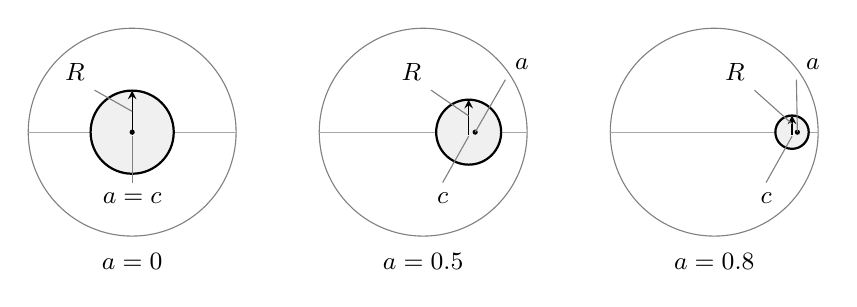
\begin{tikzpicture}[>=stealth,font=\small,scale=1.32]
 \foreach \shift/\a/\c/\rad in {0/0/0/0.4,2.8/0.5/0.4375/0.3125,5.6/0.8/0.74866/0.16043}{
  \begin{scope}[xshift=\shift cm]
   \draw[gray] (0,0) circle (1);
   \draw[gray!70] (-1,0)--(1,0);
   \draw[thick,fill=gray!12] (\c,0) circle (\rad);
   \draw[->] (\c,0)--(\c,\rad);
   \node at (\c-0.55,0.58) (radiuslabel) {\(R\)};
   \draw[gray] (radiuslabel.south east)--(\c,0.5*\rad);
   \draw (\c,-0.025)--(\c,0.025);
   \fill (\a,0) circle (0.025);
   \ifdim\a pt=0pt
    \node at (\c,-0.63) (centerlabel) {\(a=c\)};
    \draw[gray] (centerlabel.north)--(\c,-0.04);
   \else
    \node at (\c-0.25,-0.63) (centerlabel) {\(c\)};
    \draw[gray] (centerlabel.north)--(\c,-0.04);
    \node at (0.95,0.65) (pointlabel) {\(a\)};
    \draw[gray] (pointlabel.south west)--(\a,0);
   \fi
   \node[below] at (0,-1.07) {\(a=\a\)};
  \end{scope}
 }
\end{tikzpicture}
\caption[固定伪双曲半径的球]{三个圆盘都满足 \(\delta(z,a)<2/5\)，按同一欧氏尺度绘制。实心点是内在球心 \(a\)，短标记是欧氏圆心 \(c\)；第一图二者重合。由左向右，内在半径不变，欧氏半径 \(R\) 缩小，圆心差也须由公式而不是目测判断。}
\label{b3:fig:06-pseudohyperbolic-balls}
\end{figure}

\cref{b3:fig:06-pseudohyperbolic-balls}固定的是 \(r=2/5\)，而不是欧氏半径 \(R\)。在每幅图中用 \(\phi_a\) 把实心点送到原点后，小圆盘都变成同一个 \(|w|<2/5\)。

\ProseParagraphBreak

球公式给出它离单位圆的最小欧氏间隙：
\[
 1-|c|-R
 =\frac{(1-|a|)(1-r)}{1+r|a|}.
\]
对固定的 \(a,r\)，这个数为正；当中心趋向边界或半径趋向1时，它可以趋于零。因而每一个这样的闭球都是紧的，并不意味着所有闭球可被某一个共同的圆盘内紧集包住。

\ProseParagraphBreak

由距离不变性，每个圆盘自同构 \(T\) 满足
\[
 T(B_\delta(a,r))=B_\delta(T(a),r).
\]
这里等号的一个包含由 \(T\) 的不变性得到，另一个包含对 \(T^{-1}\) 使用同一性质得到。因此换坐标保留的是伪双曲半径 \(r\)，图中的欧氏半径 \(R\) 可以改变。这也解释了为什么一个自同构能在某点放大欧氏长度，同时仍保持所有伪双曲距离。

给定中心 \(a\) 的伪双曲球半径 \(r\) 增大时，欧氏中心从 \(a\) 沿径向移向0，欧氏半径增大。这不是一个固定圆心的同心圆族，却同样构成邻域基。若 \(a\) 为正实数，球与实轴的交点可直接由 \(|(x-a)/(1-ax)|=r\) 解出：
\[
 x_- =\frac{a-r}{1-ar},\quad x_+=\frac{a+r}{1+ar}.
\]
它们的平均数与半差恰为上面的 \(c,R\)，提供配方公式的另一检验。实轴上的这两个端点以后也是双曲距离计算中最简单的坐标。

\ProseParagraphBreak
这两个端点还可以量化边界附近的形状。若 \(a\in(0,1)\)，则
\[
 a-x_-=\frac{r(1-a^2)}{1-ar},\quad
 x_+-a=\frac{r(1-a^2)}{1+ar}.
\]
朝向右边界的宽度较小。当 \(a\uparrow1\) 而 \(r\) 固定时，
\[
 \frac{R}{1-a}\longrightarrow\frac{2r}{1-r^2},\quad
 \frac{1-x_+}{1-a}\longrightarrow\frac{1-r}{1+r},\quad
 \frac{1-x_-}{1-a}\longrightarrow\frac{1+r}{1-r}.
\]
所以整个小圆盘向边界收缩的尺度与 \(1-a\) 相当，但在以 \(a\) 为原点的圆盘坐标中，它始终是同一个半径 \(r\) 的盘。相反，固定 \(a\) 而令 \(r\uparrow1\) 时，\(c\to0\)、\(R\to1\)，这些球递增穷尽 \(\mathbb D\)。两种极限固定的参数不同，几何结果也不同。

\ProseParagraphBreak

现在可以证明一个容易与“距离有界”混淆的事实。

\Needspace{6\baselineskip}
\begin{proposition}\label{b3:prop:06-pseudohyperbolic-complete}
单位圆盘配备伪双曲距离 \(\delta\) 后是完备度量空间：每个 \(\delta\)-Cauchy 列都在 \(\mathbb D\) 中关于 \(\delta\) 收敛。
\end{proposition}
\begin{proof}
设 \((z_n)\) 是 \(\delta\)-Cauchy 列。取 \(N\)，使 \(m,n\ge N\) 时 \(\delta(z_m,z_n)<1/2\)。固定 \(a=z_N\)，序列尾部便包含在闭球 \(\overline B_\delta(a,1/2)\) 中。由 \cref{b3:prop:06-pseudohyperbolic-ball}，存在 \(\rho<1\)，使这个闭球包含于 \(\{|z|\le\rho\}\)。

由 \(|z_m-z_n|\le2\delta(z_m,z_n)\)，该序列是欧氏 Cauchy 列，故收敛到某个 \(z\in\mathbb C\)。尾部位于上述欧氏闭球，因而极限仍在其中，特别地 \(|z|\le\rho<1\)。再用固定紧盘上的比较式，
\[
 \delta(z_n,z)\le\frac{|z_n-z|}{1-\rho^2}\longrightarrow0
 \quad(n\ge N).
\]
这就是所需的圆盘内极限。
\end{proof}

完备性要求 Cauchy 列具有空间内极限，并不要求距离函数无界。例如取 \(z_n=1-1/n\)，\(n\ge2\)，则欧氏意义下相邻项越来越接近边界，但
\[
 \delta(z_n,z_{2n})=\frac{n}{3n-1}\longrightarrow\frac13.
\]
所以它甚至不是 \(\delta\)-Cauchy 列。这里不能只检查相邻两项的距离；Cauchy 条件要求所有充分晚的两项同时接近。闭球公式保证真正的 \(\delta\)-Cauchy 列最终留在圆盘内部的某个紧集，这正是边界点不会作为遗漏极限出现的原因。

下一节将证明任意圆盘全纯自映射都不增加 \(\delta\)。届时，不变性描述的自同构将成为压缩估计的等号情形，而本节的局部尺度公式将把两点估计转成导数估计。

% !TeX root = ../../Book3.tex
\section{Schwarz–Pick 引理}
\label{b3:sec:0603}

Schwarz 引理处理固定原点的圆盘映射。要比较任意两点，先把一个源点及其像分别送到原点，再对复合函数使用同一引理。撤销坐标后，普通的模估计就变成伪双曲距离压缩，原点导数估计则变成随位置变化的导数界。这两个结论既能判断插值数据是否相容，也能控制有内部不动点的迭代。

\subsection{Schwarz–Pick 估计与两点插值}
\label{b3:subsec:060301}

以下仍记 \(\phi_a(z)=(z-a)/(1-\overline a z)\)，其中 \(a\in\mathbb D\)。前节定义的距离为 \(\delta(z,w)=|\phi_w(z)|\)。\term[schwarz-pick-yinli]{Schwarz--Pick 引理}[Schwarz--Pick lemma]说明，全纯圆盘映射虽然未必压缩欧氏距离，却总压缩这个距离。

\Needspace{6\baselineskip}
\begin{theorem}[Schwarz--Pick]\label{b3:thm:06-schwarz-pick}
设 \(f:\mathbb D\rightarrow\mathbb D\) 全纯。则对所有 \(z,w\in\mathbb D\)，有
\[
 \delta(f(z),f(w))\le\delta(z,w),
 \quad
 \frac{|f'(w)|}{1-|f(w)|^2}\le\frac1{1-|w|^2}.
\]
若在某一点的导数不等式中取等，或在某一对不同点的距离不等式中取等，则 \(f\) 是圆盘自同构。反过来，圆盘自同构在上述所有不等式中都取等。
\end{theorem}
\begin{proof}
固定 \(w\in\mathbb D\)，令
\[
 F=\phi_{f(w)}\circ f\circ\phi_w^{-1}.
\]
两端的分式映射都是圆盘自同构，且 \(\phi_w^{-1}(0)=w\)，故 \(F:\mathbb D\rightarrow\mathbb D\) 全纯并满足 \(F(0)=0\)。Schwarz 引理给出
\[
 |F(\phi_w(z))|\le|\phi_w(z)|.
\]
左端是 \(|\phi_{f(w)}(f(z))|\)，所以这就是距离不等式。

对导数，圆盘自同构的公式给
\[
 \phi_{f(w)}'(f(w))=\frac1{1-|f(w)|^2},
 \quad (\phi_w^{-1})'(0)=1-|w|^2.
\]
于是链式法则与 Schwarz 的原点导数估计给出
\[
 |F'(0)|=
 \frac{|f'(w)|\cdot(1-|w|^2)}{1-|f(w)|^2}\le1.
\]
分母均为正，整理即得所需导数式。

若导数式取等，则 \(|F'(0)|=1\)，Schwarz 等号情形使 \(F\) 为旋转。若距离式对 \(z\ne w\) 取等，则 \(\phi_w(z)\ne0\)，同一等号情形仍使 \(F\) 为旋转。撤销两个自同构，\(f\) 便是圆盘自同构。反方向可分别对 \(f\) 和 \(f^{-1}\) 使用已证不等式，两个相反方向的估计迫使距离和导数处处取等。
\end{proof}

“不同点”的条件使距离等号具有内容；取同一点时，任何函数都会给出 \(0=0\)。常值函数也满足两个压缩式，但不在导数式或不同点的距离式中取等。若起初只有 \(|f|\le1\)，则先用最大模原理区分：\(f\) 要么是模一常值，要么处处落在开圆盘中。模一常值的分母 \(1-|f|^2\) 为零，须直接处理。

\ProseParagraphBreak

固定 \(w\)，把距离式除以 \(|z-w|\)，再令 \(z\rightarrow w\)，也会得到导数式。其分母分别趋于 \(1-|f(w)|^2\) 与 \(1-|w|^2\)。不过，一处导数界本身不会直接给出任意两点的比较；上面的坐标归一化同时控制了整个圆盘中的点值。

\Needspace{6\baselineskip}
\begin{proposition}[固定函数值的导数界]\label{b3:prop:06-value-derivative-bound}
设 \(a\in\mathbb C\)、\(R,M>0\)，\(f:D(a,R)\rightarrow D(0,M)\) 全纯，并记 \(c=f(a)\)。则
\[
 |f'(a)|\le\frac{M^2-|c|^2}{MR}.
\]
对每个 \(c\in D(0,M)\)，都存在具有该中心值并达到导数上界的映射。
\end{proposition}
\begin{proof}
在\eqref{b3:eq:06-center-derivative}中令目标圆心为零、目标半径为 \(M\)，便得所列导数界。为了确定它可以达到，任取 \(|\eta|=1\)，令
\[
 f(z)=M\cdot\phi_{c/M}^{-1}\left(\eta\frac{z-a}{R}\right).
\]
这个映射双全纯到 \(D(0,M)\)，在 \(a\) 取值 \(c\)，导数为 \(\eta(M^2-|c|^2)/(MR)\)，故达到上界。
\end{proof}

例如 \(M=R=1\)、\(a=0\)、\(c=1/2\) 时，导数模至多为 \(3/4\)，而不利用中心值的 Cauchy 估计只给 \(1\)。映射 \((z+1/2)/(1+z/2)\) 在原点的值为 \(1/2\)，导数为 \(3/4\)，说明这个改进是准确的。

\ProseParagraphBreak

两点插值把估计的必要条件变成存在性的完整判据。构造时先把第一组插值数据移到零点，余下只需用一个线性映射把第二个源值送到第二个目标值。

\Needspace{6\baselineskip}
\begin{proposition}[两点插值]\label{b3:prop:06-two-point-interpolation}
给定不同的 \(z_1,z_2\in\mathbb D\) 及 \(w_1,w_2\in\mathbb D\)。存在全纯映射 \(f:\mathbb D\rightarrow\mathbb D\)，使 \(f(z_j)=w_j\)、\(j=1,2\)，当且仅当
\[
 \delta(w_1,w_2)\le\delta(z_1,z_2).
\]
若取等，插值映射唯一，且为圆盘自同构；若严格不等，则有无穷多个不同的插值映射。
\end{proposition}
\begin{proof}
必要性来自 Schwarz--Pick。为证明充分性，令
\[
 p=\phi_{z_1}(z_2),\quad q=\phi_{w_1}(w_2),\quad c=q/p.
\]
源点互异使 \(p\ne0\)，条件又给 \(|c|\le1\)。于是
\[
 f(z)=\phi_{w_1}^{-1}\bigl(c\cdot\phi_{z_1}(z)\bigr)
\]
全纯地将圆盘映入自身，并满足两项插值。当 \(|c|=1\) 时，它是自同构。任何其他解的归一化函数 \(F=\phi_{w_1}\circ f\circ\phi_{z_1}^{-1}\) 满足 \(F(0)=0\)、\(F(p)=q\)。若 \(|q|=|p|\)，Schwarz 等号迫使 \(F(\zeta)=c\zeta\)，所以这个解唯一。

若 \(|c|<1\)，对每个满足
\[
 |t|<\frac{1-|c|}{1+|p|}
\]
的复数 \(t\)，定义 \(H_t(\zeta)=c+t(\zeta-p)\)。对 \(\zeta\in\mathbb D\)，有 \(|H_t(\zeta)|\le|c|+|t|\cdot(1+|p|)<1\)，而 \(H_t(p)=c\)。因此 \(F_t(\zeta)=\zeta\cdot H_t(\zeta)\) 都满足 \(F_t(0)=0\)、\(F_t(p)=q\)。撤销坐标得到插值映射 \(f_t\)。不同的 \(t\) 给出不同的多项式 \(F_t\)，故也给出不同的 \(f_t\)。
\end{proof}

取 \(z_1=w_1=0\)、\(z_2=1/2\)。若要求 \(w_2=3/4\)，目标距离大于源距离，无解；若改为 \(w_2=1/4\)，则 \(f(z)=z/2\) 是一个解；若取 \(w_2=1/2\)，唯一解是恒等映射。对三个点，原始数据的成对距离条件还不够，下一小节将用一次除零点步骤找出剩余的相容条件。

\ProseParagraphBreak

严格压缩不意味着全圆盘共有一个小于 \(1\) 的压缩系数。对 \(f(z)=z^2\)，其归一化导数比为
\[
 \frac{|f'(z)|\cdot(1-|z|^2)}{1-|f(z)|^2}
 =\frac{2|z|}{1+|z|^2}<1.
\]
每个内点都严格小于 \(1\)，但沿 \(|z|\uparrow1\) 趋于 \(1\)。只有固定 \(|z|\le r<1\) 后，才能用 \(2r/(1+r^2)<1\) 作共同上界。

\subsection{不动点迭代与插值构造}
\label{b3:subsec:060302}

圆盘映射若有内部不动点，就可以通过共轭把它移到原点。此时 Schwarz 引理使每条轨道留在一个内部紧盘里，紧盘上的严格性足以证明整条迭代轨道收敛。

\Needspace{6\baselineskip}
\begin{proposition}[内部不动点的刚性]\label{b3:prop:06-two-fixed-points}
设 \(f:\mathbb D\rightarrow\mathbb D\) 全纯。若 \(f\) 固定两个不同的内部点，则 \(f\) 为恒等映射。若 \(a\in\mathbb D\)、\(f(a)=a\) 且 \(f'(a)=1\)，则 \(f\) 也为恒等映射。
\end{proposition}
\begin{proof}
若有两个不同不动点 \(a,b\)，距离不等式在该点对取等，故 \(f\) 是自同构。映射 \(g=\phi_a\circ f\circ\phi_a^{-1}\) 固定零点，所以是旋转 \(g(\zeta)=\eta\zeta\)。它还固定非零点 \(\phi_a(b)\)，故 \(\eta=1\)，撤销共轭即得 \(f=\mathrm{id}\)。

对第二项，同样的共轭满足 \(g(0)=0\)，并由链式法则得到 \(g'(0)=f'(a)=1\)。Schwarz 导数等号给出 \(g(\zeta)=\zeta\)，于是 \(f\) 仍是恒等映射。
\end{proof}

\Needspace{6\baselineskip}
\begin{proposition}[内点不动点处的迭代]\label{b3:prop:06-interior-iteration}
设 \(f:\mathbb D\rightarrow\mathbb D\) 全纯，\(a\in\mathbb D\)，且 \(f(a)=a\)。若 \(f\) 不是圆盘自同构，则迭代 \(f^{\circ n}\) 在 \(\mathbb D\) 上局部一致趋于常值 \(a\)。在已有内部不动点的条件下，\(f\) 不是圆盘自同构等价于 \(|f'(a)|<1\)。
\end{proposition}
\begin{proof}
令 \(g=\phi_a\circ f\circ\phi_a^{-1}\)。它固定零点，且 \(g'(0)=f'(a)\)。Schwarz 引理给 \(|g'(0)|\le1\)，取等当且仅当 \(g\) 为旋转；这也恰是 \(f\) 为圆盘自同构的情形。因此题设等价于 \(|f'(a)|<1\)。

在原点补上导数后，函数 \(h(\zeta)=g(\zeta)/\zeta\) 全纯且 \(|h|\le1\)。若它在某个内点取模 \(1\)，最大模原理使它为单位常数，\(g\) 就成为旋转，与假设矛盾。所以对每个 \(0<r<1\)，都有
\[
 q_r=\max_{|\zeta|\le r}|h(\zeta)|<1.
\]
Schwarz 引理使 \(g\) 把 \(\overline{D(0,r)}\) 映入自身，故可反复使用同一个常数，归纳得到
\[
 |g^{\circ n}(\zeta)|\le q_r^n\cdot|\zeta|
 \quad(|\zeta|\le r).
\]
对原圆盘中的固定紧集 \(K\)，选 \(r<1\) 使 \(\phi_a(K)\subseteq\overline{D(0,r)}\)。因为
\[
 \phi_a^{-1}(u)-a=\frac{(1-|a|^2)u}{1+\overline a u},
\]
共轭关系给出
\[
 \sup_{z\in K}|f^{\circ n}(z)-a|
 \le\frac{1-|a|^2}{1-|a|\cdot r}\,q_r^n r
 \longrightarrow0.
\]
分母为正，且不随 \(n\) 改变，故得到紧集上的一致收敛。
\end{proof}

旋转是这一结论的准确例外。若共轭后的映射为 \(g(\zeta)=\eta\zeta\)、\(|\eta|=1\)，则迭代为 \(\eta^n\zeta\)。当 \(\eta\ne1\) 时，任何非零轨道都不收敛：若极限为 \(L\)，其模非零，而相邻项关系又给 \(L=\eta L\)，矛盾。单位根情形的轨道是周期的；\(\eta=1\) 时则每个点固定。没有内部不动点的映射可能有趋近边界的轨道，那属于后续 Denjoy--Wolff 理论，本处不据此作结论。

\ProseParagraphBreak

例如 \(g(z)=z^2\) 的第 \(n\) 次迭代为 \(z^{2^n}\)，在 \(|z|\le r<1\) 上误差至多 \(r^{2^n}\)，却不在整个开圆盘上一致趋于零，其模的全域上确界始终为 \(1\)。固定紧集使所有迭代点共享一个严格小于 \(1\) 的估计。

\ProseParagraphBreak

把归一化后的零点除去，也能逐步处理插值数据。一次取值条件被消去以后，剩余自由度由另一个模不超过 \(1\) 的全纯函数表示。这称为\term[schur-buzhou]{Schur 步骤}[Schur step]。

\Needspace{6\baselineskip}
\begin{proposition}[Schur 步骤]\label{b3:prop:06-schur-step}
给定 \(c\in\mathbb D\)，令 \(\phi_c(w)=(w-c)/(1-\overline c w)\)。若 \(f:\mathbb D\rightarrow\mathbb D\) 全纯且 \(f(0)=c\)，则
\[
 g(z)=\frac{\phi_c(f(z))}{z}\quad(z\ne0)
\]
在原点可去，补定义后全纯且 \(|g(z)|\le1\)，并有
\[
 g(0)=\frac{f'(0)}{1-|c|^2}.
\]
反过来，对每个在 \(\mathbb D\) 上全纯且模不超过 \(1\) 的函数 \(g\)，公式
\[
 f(z)=\phi_c^{-1}\bigl(z\cdot g(z)\bigr)
     =\frac{c+z\cdot g(z)}{1+\overline c z\cdot g(z)}
\]
定义一个满足 \(f(0)=c\) 的全纯圆盘映射。这两个操作互为逆操作。
\end{proposition}
\begin{proof}
函数 \(\phi_c\circ f\) 固定零点，Schwarz 引理给 \(|\phi_c(f(z))|\le|z|\)。其 Taylor 展开的一次系数为 \(\phi_c'(c)\cdot f'(0)=f'(0)/(1-|c|^2)\)，所以除以 \(z\) 后可去，且原点补值如上。模估计在非零点成立，在原点由连续性成立。

反过来，\(|z\cdot g(z)|\le|z|<1\)，因此即使 \(g\) 是单位常数，乘积也始终落在开圆盘内。分母的模至少为 \(1-|c|\cdot|z|>0\)，复合逆自同构合法，给出全纯圆盘映射及 \(f(0)=c\)。两边施加 \(\phi_c\) 得到 \(\phi_c(f(z))=z\cdot g(z)\)，从而两个操作互逆。
\end{proof}

如果 \(|f'(0)|=1-|c|^2\)，则 \(|g(0)|=1\)，最大模原理迫使 \(g\) 是单位常数，原函数因而是自同构。若 \(|g(0)|<1\)，则 \(g\) 全部取值于开盘，才可继续作下一步。例如 \(f(0)=f'(0)=0\) 时，连续两次 Schwarz 除零点得到 \(|f(z)|\le|z|^2\)；若再有 \(f''(0)=2\eta\)、\(|\eta|=1\)，第二个商被迫恒为 \(\eta\)，所以 \(f(z)=\eta z^2\)。

\Needspace{6\baselineskip}
\begin{proposition}[二阶 Taylor 数据的相容性]\label{b3:prop:06-second-jet}
给定 \(c,d,e\in\mathbb C\)、\(|c|<1\)，记
\[
 A=1-|c|^2,\quad p=\frac dA,\quad
 q=\frac eA+\frac{\overline c d^2}{A^2}.
\]
存在全纯映射 \(f:\mathbb D\rightarrow\mathbb D\)，使其原点展开为
\[
 f(z)=c+dz+ez^2+O(z^3),
\]
当且仅当以下两种情形之一成立：\(|p|<1\) 且 \(|q|\le1-|p|^2\)；或者 \(|p|=1\) 且 \(q=0\)。这里 \(e=f''(0)/2\)。
\end{proposition}
\begin{proof}
先作 Schur 步骤，令 \(g=\phi_c(f)/z\)。为了辨认 \(g\) 的前两项，记 \(t=f-c=dz+ez^2+O(z^3)\)。因为 \(A>0\)，原点附近有
\[
 \begin{aligned}
 \phi_c(f)&=\frac{t}{A-\overline c t}
   =\frac tA+\frac{\overline c}{A^2}t^2+O(z^3)\\
 &=\frac dA z+
   \left(\frac eA+\frac{\overline c d^2}{A^2}\right)z^2+O(z^3).
 \end{aligned}
\]
所以 \(g(z)=p+qz+O(z^2)\)。Schur 步骤给 \(|g|\le1\)，先有 \(|p|\le1\)。若 \(|p|=1\)，最大模原理使 \(g\equiv p\)，故 \(q=0\)。若 \(|p|<1\)，最大模原理排除其他点取模 \(1\)，于是 \(g\) 是开圆盘自映射，Schwarz--Pick 在原点给出 \(|q|\le1-|p|^2\)。这证明了必要性。

为证明充分性，若 \(|p|<1\)，令
\[
 k=\frac q{1-|p|^2},\quad
 g(z)=\phi_p^{-1}(kz)=\frac{p+kz}{1+\overline p kz}.
\]
条件保证 \(|k|\le1\)，所以 \(g\) 把开圆盘映入开圆盘，且 \(g(0)=p\)、\(g'(0)=(1-|p|^2)k=q\)。若 \(|p|=1\)、\(q=0\)，则取 \(g\equiv p\)。两种情形都可以令 \(f=\phi_c^{-1}(zg)\)，Schur 逆步骤保证 \(f:\mathbb D\rightarrow\mathbb D\) 全纯。

还须核对恢复的二阶项。逆分式在零点附近展开为
\[
 \phi_c^{-1}(u)=c+A u-A\overline c u^2+O(u^3).
\]
代入 \(u=z\cdot g(z)=pz+qz^2+O(z^3)\)，得到
\[
 f(z)=c+A pz+A(q-\overline c p^2)z^2+O(z^3).
\]
定义给出 \(Ap=d\)、\(A(q-\overline c p^2)=e\)，因此所构造函数具有全部指定数据。
\end{proof}

当 \(c=0\) 时，条件变成 \(|d|\le1\)、\(|e|\le1-|d|^2\)。例如 \(d=3/4\)、\(e=1/2\) 不相容，因为 \(1/2>7/16\)，尽管两个系数单独都满足 Cauchy 的模上界 \(1\)。当 \(c=1/2\)、\(d=3/4\) 时，第一步已经给 \(p=1\)，于是 \(q=0\) 强制 \(e=-3/8\)。这正是 \((z+1/2)/(1+z/2)\) 的二次系数，显示分式归一化中的 \(\overline c d^2\) 项不可丢掉。

\ProseParagraphBreak

三点插值也能通过一次 Schur 步骤变成两点问题。除零点后出现的指定值可能位于单位圆上，因此需要先处理这个边界情形，再使用开圆盘中的两点判据。

\Needspace{6\baselineskip}
\begin{proposition}[三点插值的 Schur 归约]\label{b3:prop:06-three-point-reduction}
设 \(a_1,a_2,a_3\in\mathbb D\) 两两不同，\(b_1,b_2,b_3\in\mathbb D\)。记 \(\phi_a(z)=(z-a)/(1-\overline a z)\)，并令
\[
 p_j=\phi_{a_1}(a_j),\quad
 q_j=\frac{\phi_{b_1}(b_j)}{p_j}\quad(j=2,3).
\]
存在全纯映射 \(f:\mathbb D\rightarrow\mathbb D\)，使 \(f(a_j)=b_j\)、\(j=1,2,3\)，当且仅当以下之一成立：\(q_2,q_3\in\mathbb D\) 且 \(\delta(q_2,q_3)\le\delta(p_2,p_3)\)；或者 \(q_2=q_3\) 且 \(|q_2|=1\)。
\end{proposition}
\begin{proof}
源点互异使 \(p_2,p_3\) 非零且不同，故各商有定义。若插值映射存在，则
\[
 G=\phi_{b_1}\circ f\circ\phi_{a_1}^{-1}
\]
是固定零点的圆盘映射。Schur 步骤使 \(H(\zeta)=G(\zeta)/\zeta\) 在零点可去，且 \(|H|\le1\)。插值条件等价于 \(H(p_j)=q_j\)、\(j=2,3\)。如果某个 \(|q_j|>1\)，便不可能；如果某个 \(|q_j|=1\)，最大模原理迫使 \(H\) 恒为这个单位数，所以另一个 \(q_j\) 必须相同。剩下 \(q_2,q_3\in\mathbb D\) 的情形，\(H\) 也处处在开盘内，两点插值判据给出所列距离条件。

反过来，若 \(q_2=q_3\) 为单位数，取 \(H\equiv q_2\)。若两值都在开盘且满足距离条件，可以明确取
\[
 k=\frac{\phi_{q_2}(q_3)}{\phi_{p_2}(p_3)},
 \quad H(\zeta)=\phi_{q_2}^{-1}\bigl(k\cdot\phi_{p_2}(\zeta)\bigr).
\]
因为 \(p_2\ne p_3\)，分母非零，而条件给 \(|k|\le1\)。这就是两点命题中的构造，满足 \(H(p_j)=q_j\)。两种情形均可定义
\[
 f(z)=\phi_{b_1}^{-1}\Bigl(
       \phi_{a_1}(z)\cdot H\bigl(\phi_{a_1}(z)\bigr)\Bigr).
\]
乘积的模严格小于 \(1\)，包括 \(H\) 为单位常数的情形，故所得函数全纯且取值于开盘。在 \(a_1\) 处乘积为零；在另外两点处，它等于 \(p_jq_j=\phi_{b_1}(b_j)\)。代入逆分式就恢复全部三项插值。
\end{proof}

若约化函数被迫为单位常数，或最后两点的距离不等式取等，约化后的 \(H\) 唯一，原映射也唯一。若最后两点严格不等，前面的构造给出无穷多个不同的 \(H\)，逆步骤也给出不同的原映射。

\ProseParagraphBreak

例如要求 \(f(0)=0\)、\(f(1/2)=f(-1/2)=2/5\)。每一对原始数据都满足 Schwarz--Pick：中心到另外两点的目标距离为 \(2/5<1/2\)，后两个目标之间的距离为零。但除去已知零点后，\(H=f/z\) 必须在 \(1/2,-1/2\) 分别取值 \(4/5,-4/5\)。这不可能，因为
\[
 \delta(4/5,-4/5)=\frac{40}{41}
 >\frac45=\delta(1/2,-1/2).
\]
共同的 Schur 归约揭示了各点数据之间的额外约束，不能把不同点对各自存在的解直接拼接。

\subsection{等号刚性与正实部估计}
\label{b3:subsec:060303}

内部的精确等号已经迫使映射成为自同构；若导数只是接近极值，还可以量化函数在紧集上离极端映射有多远。设 \(f:\mathbb D\rightarrow\mathbb D\) 全纯，\(f(0)=0\)，且 \(f'(0)=a\in[0,1]\)。当 \(a<1\) 时，商 \(h=f/z\) 补定义后满足 \(h(0)=a\)、\(|h|<1\)。Schwarz--Pick 给 \(\delta(h(z),a)\le|z|\)。固定 \(0<r<1\)，对 \(|z|\le r\) 有
\[
 \begin{aligned}
 |h(z)-a|&\le r\cdot|1-ah(z)|\\
 &\le r\bigl(1-a^2+a\cdot|h(z)-a|\bigr).
 \end{aligned}
\]
因为 \(1-ar>0\)，移项给出 \(|h-a|\le r(1-a^2)/(1-ar)\)。再由 \(|f(z)-z|\le|z|\cdot(|h(z)-a|+1-a)\)，得到
\[
 \sup_{|z|\le r}|f(z)-z|
 \le\frac{r(1-a)(1+r)}{1-ar}.
\]
若 \(a=1\)，Schwarz 等号直接给 \(f=z\)，同一上界仍成立。因此归一化导数趋于 \(1\) 时，函数在每个固定紧盘上一致趋于恒等。对非零复导数，可先旋转函数使导数正实，再与相应旋转映射比较。

\ProseParagraphBreak

把右半平面映到圆盘，还能将正实部条件转成模约束。这个转换保留的信息比一般的模有界条件更强，因为实部的正性同时控制了圆周平均值和各阶系数。

\Needspace{6\baselineskip}
\begin{proposition}[正实部函数的增长估计]\label{b3:prop:06-positive-real-part}
设 \(p:\mathbb D\rightarrow\mathbb C\) 全纯，\(\operatorname{Re}p(z)>0\) 对全部 \(z\in\mathbb D\) 成立，且 \(p(0)=1\)。则对每个 \(z\in\mathbb D\)，记 \(r=|z|\)，有
\[
 \frac{1-r}{1+r}\le\operatorname{Re}p(z)
 \le\frac{1+r}{1-r},
 \quad |p(z)|\le\frac{1+r}{1-r}.
\]
\end{proposition}
\begin{proof}
正实部使 \(p+1\) 无零，且
\[
 |p+1|^2-|p-1|^2=4\operatorname{Re}p>0.
\]
所以 \(q=(p-1)/(p+1)\) 是圆盘映射，\(q(0)=0\)，Schwarz 引理给 \(|q(z)|\le r\)。反解 \(p=(1+q)/(1-q)\)，得到
\[
 \operatorname{Re}p(z)=\frac{1-|q(z)|^2}{|1-q(z)|^2}.
\]
令 \(s=|q(z)|\le r\)。由 \(1-s\le|1-q(z)|\le1+s\)，有
\[
 \frac{1-s}{1+s}\le\operatorname{Re}p(z)\le\frac{1+s}{1-s},
 \quad |p(z)|\le\frac{1+s}{1-s}.
\]
左侧函数随 \(s\) 递减，右侧函数随 \(s\) 递增，代入 \(s\le r\) 即得全部估计。
\end{proof}

函数 \(p_\eta(z)=(1+\eta z)/(1-\eta z)\)、\(|\eta|=1\)，在满足 \(\eta z=r\) 的点达到上界，在满足 \(\eta z=-r\) 的点达到实部下界。因此两个方向的界都可达到。这里的推导只对全纯函数的实部进行，后面的调和函数理论将解释同样的 Harnack 因子。

\ProseParagraphBreak

\term[caratheodory-xishu-budengshi]{Carathéodory 系数不等式}[Carathéodory coefficient inequality]进一步给出与阶数无关的系数界。

\Needspace{6\baselineskip}
\begin{proposition}[Carathéodory 系数估计]\label{b3:prop:06-caratheodory-coefficients}
设 \(p:\mathbb D\rightarrow\mathbb C\) 全纯，\(\operatorname{Re}p>0\)、\(p(0)=1\)，且
\[
 p(z)=1+\sum_{n=1}^{\infty}c_nz^n.
\]
则每个整数 \(n\ge1\) 都满足 \(|c_n|\le2\)。
\end{proposition}
\begin{proof}
固定 \(0<r<1\)，记 \(u(t)=\operatorname{Re}p(re^{\mathrm{i}t})>0\)。Taylor 级数在这一固定圆周上一致收敛，故可取实部，写为
\[
 u(t)=1+\frac12\sum_{m=1}^{\infty}
 \left(c_mr^me^{\mathrm{i}mt}+\overline{c_m}r^me^{-\mathrm{i}mt}\right).
\]
对这个一致收敛级数逐项积分，利用非零整数频率的指数在一周上的积分为零，得到
\[
 \frac1{2\pi}\int_0^{2\pi}u(t)\,\mathrm{d}t=1,
 \quad
 \frac1{2\pi}\int_0^{2\pi}u(t)\cdot e^{-\mathrm{i}nt}\,\mathrm{d}t
 =\frac12c_nr^n\quad(n\ge1).
\]
因为 \(u(t)>0\) 且 \(|e^{-\mathrm{i}nt}|=1\)，带振荡因子的积分模不超过 \(u\) 的积分。因此 \(|c_n|\cdot r^n\le2\)。对固定 \(n\) 令 \(r\uparrow1\)，得到 \(|c_n|\le2\)。整个论证只在内部圆周上积分，不需要 \(p\) 在单位圆上具有边界值。
\end{proof}

上面的极端函数还有展开
\[
 \frac{1+\eta z}{1-\eta z}
 =1+2\sum_{n=1}^{\infty}\eta^nz^n\quad(|\eta|=1),
\]
所有非恒定系数的模均为 \(2\)，所以每个阶数都达到同一界。若全纯函数 \(p(z)=c_0+\sum_{n\ge1}c_nz^n\) 仍满足 \(\operatorname{Re}p>0\)，但常数项任意，令 \(\alpha=\operatorname{Re}c_0>0\)、\(\beta=\operatorname{Im}c_0\)。归一化函数 \((p-\mathrm{i}\beta)/\alpha\) 满足前一命题，故一般形式为 \(|c_n|\le2\operatorname{Re}c_0\)、\(n\ge1\)。常数项的虚部不参与这个约束。

\subsection{共形映射下的转移}
\label{b3:subsec:060304}

对真单连通区域，Riemann 映照提供全局圆盘坐标。先把距离和局部尺度转回原区域，并证明它们不依赖坐标选择，就能将 Schwarz--Pick 写成区域本身的结论。

\Needspace{6\baselineskip}
\begin{definition}[区域上的距离与密度]\label{b3:def:06-conformal-transfer}
设 \(U\subsetneq\mathbb C\) 为单连通区域，\(\Phi:U\rightarrow\mathbb D\) 为双全纯映射。对 \(z,w\in U\)，定义
\[
 \delta_U(z,w)\coloneqq\delta(\Phi(z),\Phi(w)),
 \quad
 \lambda_U(z)\coloneqq\frac{2|\Phi'(z)|}{1-|\Phi(z)|^2}.
\]
分别称为 \(U\) 上的伪双曲距离和\term[poincare-midu]{Poincaré 密度}[Poincaré density]。
\end{definition}
\symidx{\(\delta_U(z,w)\)：真单连通区域上的伪双曲距离}
\symidx{\(\lambda_U(z)\)：Poincaré 密度}

这两个定义与 \(\Phi\) 的选择无关。若另一坐标为 \(\Psi\)，则 \(A=\Psi\circ\Phi^{-1}\) 是圆盘自同构，前节的不变性给出 \(\delta(Au,Av)=\delta(u,v)\)。同时，自同构的导数恒等式为
\[
 \frac{|A'(u)|}{1-|A(u)|^2}=\frac1{1-|u|^2}.
\]
代入 \(u=\Phi(z)\) 并使用链式法则，便得用 \(\Psi\) 和用 \(\Phi\) 计算的 \(\lambda_U\) 相同。距离的度量性质由双射 \(\Phi\) 和 \(\delta\) 的性质传回；密度则处处为正，因为双全纯映射的导数不为零。

\ProseParagraphBreak

密度与上一章的共形半径可以在基点处直接比较。对固定 \(a\in U\)，选择满足 \(\Phi(a)=0\)、\(\Phi'(a)>0\) 的归一化坐标，得到
\[
 \lambda_U(a)=2\Phi'(a)=\frac2{r_U(a)}.
\]
坐标无关性保证这个等式对每个基点都成立。

\Needspace{6\baselineskip}
\begin{proposition}[单连通区域上的 Schwarz--Pick 估计]\label{b3:prop:06-conformal-schwarz-pick}
设 \(U,V\subsetneq\mathbb C\) 为单连通区域，\(f:U\rightarrow V\) 全纯。则对所有 \(z,w\in U\)，有
\[
 \delta_V(f(z),f(w))\le\delta_U(z,w),
 \quad \lambda_V(f(z))\cdot|f'(z)|\le\lambda_U(z).
\]
若在一对不同点的距离式中取等，或在某一点的导数式中取等，则 \(f\) 双全纯映满 \(V\)。反过来，双全纯映射在这些式子中处处取等。
\end{proposition}
\begin{proof}
取圆盘坐标 \(\Phi_U:U\rightarrow\mathbb D\)、\(\Phi_V:V\rightarrow\mathbb D\)，并令 \(G=\Phi_V\circ f\circ\Phi_U^{-1}\)。圆盘的 Schwarz--Pick 距离式直接变成所需的距离式。对 \(a\in U\)，在 \(\zeta=\Phi_U(a)\) 处有
\[
 G'(\zeta)=\frac{\Phi_V'(f(a))\cdot f'(a)}{\Phi_U'(a)}.
\]
将它代入圆盘导数式，再乘以正数 \(2|\Phi_U'(a)|\)，便得到 \(\lambda_V(f(a))\cdot|f'(a)|\le\lambda_U(a)\)。这里坐标导数均非零，所有分母为正，所以等号也准确对应。圆盘中的等号迫使 \(G\) 为自同构，故 \(f=\Phi_V^{-1}\circ G\circ\Phi_U\) 双全纯映满 \(V\)。反向同样由圆盘自同构的等号性质得到。
\end{proof}

用共形半径改写导数式，就是
\[
 \frac{|f'(a)|}{r_V(f(a))}\le\frac1{r_U(a)}.
\]
若 \(U\subseteq V\)，对恒等嵌入应用此式，得到 \(r_U(a)\le r_V(a)\)；一处取等就迫使恒等嵌入满射，所以只能有 \(U=V\)。这也恢复了上一章共形半径的严格单调性。

\ProseParagraphBreak

在右半平面 \(H_R=\{\,z\in\mathbb C\mid\operatorname{Re}z>0\,\}\)，取 \(\Phi(z)=(z-1)/(z+1)\)。由
\[
 |\Phi'(z)|=\frac2{|z+1|^2},
 \quad 1-|\Phi(z)|^2=\frac{4\operatorname{Re}z}{|z+1|^2},
\]
可得 \(\lambda_{H_R}(z)=1/\operatorname{Re}z\)。因此每个全纯映射 \(F:\mathbb D\rightarrow H_R\) 满足
\[
 \frac{|F'(z)|}{\operatorname{Re}F(z)}\le\frac2{1-|z|^2}.
\]
若 \(F(0)=1\)，距离式还给 \(|(F(z)-1)/(F(z)+1)|\le|z|\)，正是前面正实部估计所使用的圆盘约束。

\ProseParagraphBreak

在上半平面 \(\mathbb H=\{\,z\in\mathbb C\mid\operatorname{Im}z>0\,\}\)，同样用 \((z-\mathrm{i})/(z+\mathrm{i})\) 计算，得到
\[
 \delta_{\mathbb H}(z,w)=\left|\frac{z-w}{z-\overline w}\right|,
 \quad \lambda_{\mathbb H}(z)=\frac1{\operatorname{Im}z}.
\]
于是全纯映射 \(F:\mathbb H\rightarrow\mathbb H\) 满足
\[
 \left|\frac{F(z)-F(w)}{F(z)-\overline{F(w)}}\right|
 \le\left|\frac{z-w}{z-\overline w}\right|,
 \quad \frac{|F'(z)|}{\operatorname{Im}F(z)}\le\frac1{\operatorname{Im}z}.
\]
例如 \(F(z)=z+\mathrm{i}\) 的欧氏导数为 \(1\)，但 \(\operatorname{Im}F(z)=\operatorname{Im}z+1\)，所以密度导数式严格压缩。若 \(F(z)=(az+b)/(cz+d)\)，其中 \(a,b,c,d\) 为实数、\(ad-bc>0\)，则
\[
 \operatorname{Im}F(z)=\frac{(ad-bc)\operatorname{Im}z}{|cz+d|^2}.
\]
它及其分式逆都保持上半平面，故为自同构，在两个估计中均取等。

\ProseParagraphBreak

本小节的全局圆盘坐标依赖真单连通条件。对有孔区域，局部坐标不能直接拼成一个双全纯圆盘映射，推广密度需要后面的覆盖理论。\chapref{b3:ch:13}还将用 \(\lambda_U(z)\cdot|\mathrm{d}z|\) 定义曲线长度，再由长度下确界构造 Poincaré 距离；这里的 \(\delta_U\) 与那个路径距离是不同的数值。


\begin{chaptersummary}
本章反复使用同一个归一化方法：先把指定的源点和像点送到0，再对所得圆盘映射应用 Schwarz 引理。撤销坐标后，函数值的比较成为伪双曲距离压缩，导数的比较则带上源、目标两处的密度因子。伪双曲距离虽小于1，仍是真正的度量；其球的欧氏大小随位置变化，固定内部紧集上的欧氏比较不能直接推广到圆盘边缘。

\ProseParagraphBreak

精确等号与定量压缩承担不同任务。一对不同内点或一个内点导数的等号迫使自同构；非自同构给逐点严格不等式，却未必给全域共有的小于1的系数。有限零点除法与 Schur 步骤把这一思想用于系数和插值：先化去已给数据，再检查剩余函数是否仍满足圆盘约束，最后反向构造。正实部问题通过 Cayley 变换接入同一方法。换到一般真单连通区域时，距离与密度不依赖所选圆盘坐标；显式的半平面和条带计算说明这种不变性怎样变成可用的尺度估计。
\end{chaptersummary}

\BookExercises

% 本章8题均为自拟；以已有工具增加边界尺度、球几何、插值构造和显式迭代训练。
\Needspace{6\baselineskip}
\begin{exercise}\label{b3:ex:06-1}
对 \(0<r<1\)，计算 \(\delta(r,-r)\) 与 \(\delta(0,r)\)，比较它们与对应的欧氏距离。再固定 \(\alpha,\beta>0\)，令
\[
 z_\varepsilon=1-\alpha\varepsilon,\quad
 w_\varepsilon=1-\beta\varepsilon
\]
在充分小的 \(\varepsilon>0\) 时位于单位圆盘内，求 \(\delta(z_\varepsilon,w_\varepsilon)\) 的极限。最后考察 \(z_n=1-1/n\)、\(w_n=1-1/n^2\)，说明两个点即使趋于同一个边界点、欧氏距离趋于0，伪双曲距离也可能趋于1。
\end{exercise}
\begin{solution}
由定义直接得到
\[
 \delta(r,-r)=\frac{2r}{1+r^2},
 \quad
 \delta(0,r)=r.
\]
对应的欧氏距离是 \(2r\) 与 \(r\)。第一组中伪双曲距离小于欧氏距离，两组伪双曲距离都在 \(r\uparrow1\) 时趋于1；这些计算并不说明在所有位置都能用欧氏距离给统一的上界。

取 \(0<\varepsilon<1/\max\{\alpha,\beta\}\)，两个点均为 \((0,1)\) 中的实数，且
\[
 1-z_\varepsilon w_\varepsilon
 =(\alpha+\beta)\varepsilon-\alpha\beta\varepsilon^2>0.
\]
于是
\[
 \delta(z_\varepsilon,w_\varepsilon)
 =\frac{|\alpha-\beta|}{\alpha+\beta-\alpha\beta\varepsilon}
 \longrightarrow\frac{|\alpha-\beta|}{\alpha+\beta}.
\]
若 \(\alpha\ne\beta\)，极限为正，而欧氏距离
\(|z_\varepsilon-w_\varepsilon|=|\alpha-\beta|\varepsilon\) 趋于0。因此不存在一个对全单位圆盘有效的有限常数 \(C\)，使 \(\delta(z,w)\le C|z-w|\) 对全部点成立。这里两点离边界的距离具有同一阶，极限记录的是两个尺度的比值。

若靠近边界的速度不同，距离还能更大。对 \(n\ge2\)，
\[
 \delta(z_n,w_n)
 =\frac{1/n-1/n^2}{1/n+1/n^2-1/n^3}
 =\frac{n^2-n}{n^2+n-1}\longrightarrow1.
\]
与此同时，\(|z_n-w_n|=1/n-1/n^2\to0\)，且两点都趋于1。伪双曲距离所保留的分母与两点各自的边界尺度有关，不能只凭欧氏图上的靠近判断其极限。
\end{solution}

\Needspace{6\baselineskip}
\begin{exercise}\label{b3:ex:06-2}
不直接套用一般球公式，从不等式出发求
\[
 B=\{\,z\in\mathbb D\mid\delta(z,1/2)<1/2\,\}
\]
的欧氏中心、半径及与实轴的交点。用自同构 \(\phi_{1/2}\) 解释这两个端点，并求闭球 \(\overline B\) 到单位圆周的最短欧氏距离。说明为什么伪双曲球心 \(1/2\) 不是这个欧氏圆盘的中心。
\end{exercise}
\begin{solution}
令 \(z=x+\mathrm{i}y\)。由于 \(1-z/2\ne0\)，球条件等价于
\[
 |z-1/2|^2<\frac14|1-z/2|^2.
\]
两边展开并移项，得到
\[
 \frac{15}{16}(x^2+y^2)-\frac34x<0,
\]
再除以首项系数并配方：
\[
 \left(x-\frac25\right)^2+y^2<\left(\frac25\right)^2.
\]
因此欧氏圆心为 \(2/5\)，半径为 \(2/5\)。这个圆盘确实包含于单位圆盘，因为其闭包上的 \(|z|\) 至多为 \(4/5<1\)。它与实轴的交集为 \((0,4/5)\)，两个边界端点为0和 \(4/5\)。

从自同构看，\(\phi_{1/2}\) 把 \(B\) 送到 \(|\zeta|<1/2\)，并把内在球心 \(1/2\) 送到0。它的逆式是
\[
 \phi_{1/2}^{-1}(\zeta)=\frac{\zeta+1/2}{1+\zeta/2}.
\]
代入 \(\zeta=-1/2\) 和 \(\zeta=1/2\)，分别得到0和 \(4/5\)。所以两个实轴端点是同一条直径两端的逆像。分式映射不保持欧氏中点：它们的中点为 \(2/5\)，而0在逆映射下的像为 \(1/2\)。从 \(1/2\) 到两端的欧氏距离分别为 \(1/2\) 与 \(3/10\)，但两端到 \(1/2\) 的伪双曲距离都为 \(1/2\)。

对单位圆盘内任意点 \(z\)，它到单位圆周的欧氏距离是 \(1-|z|\)。闭球中最大的 \(|z|\) 为 \(4/5\)，在正实点 \(4/5\) 达到。因此闭球到单位圆周的最短距离为
\[
 1-\frac45=\frac15,
\]
由 \(4/5\) 与1这对点实现。计算这个正间隙，也就具体核对了该闭伪双曲球是单位圆盘内的紧集。
\end{solution}

\Needspace{6\baselineskip}
\begin{exercise}\label{b3:ex:06-3}
设 \(f:\mathbb D\rightarrow\mathbb D\) 全纯，且
\[
 f(z)=\frac12+\frac12z+ez^2+O(z^3).
\]
求全部允许的二次系数 \(e\in\mathbb C\)，通过 Schur 步骤给出每个允许值对应函数的构造，并证明当 \(e\) 位于允许系数域的边界上时，满足这些数据的函数唯一。
\end{exercise}
\begin{solution}
先将常数项送到0，再除去原点零点：
\[
 g(z)=\frac1z\cdot\frac{f(z)-1/2}{1-f(z)/2}.
\]
Schwarz 引理说明该式在0可去，且 \(|g|\le1\)。为确定留下的数据，实际展开分式：
\[
 \frac{f(z)-1/2}{1-f(z)/2}
 =\frac{\frac12z+ez^2+O(z^3)}
        {\frac34-\frac14z-\frac12ez^2+O(z^3)}
 =\frac23z+\left(\frac43e+\frac29\right)z^2+O(z^3).
\]
所以
\[
 g(0)=\frac23,\quad g'(0)=q=\frac43e+\frac29.
\]
由于 \(g(0)\) 在开圆盘内，最大模原理排除单位常数情形，故 \(g:\mathbb D\to\mathbb D\)。原点处的 Schwarz--Pick 导数式给
\[
 |q|\le1-\frac49=\frac59.
\]
这等价于
\[
 \left|e+\frac16\right|\le\frac5{12}.
\]
可见允许系数域是一个以 \(-1/6\) 为中心的闭圆盘，而不是以0为中心的独立 Cauchy 系数界。

反过来，给定满足该条件的 \(e\)，置
\[
 \kappa=\frac95q=\frac{12e+2}{5},\quad |\kappa|\le1,
\]
并定义
\[
 g_\kappa(z)=\frac{2/3+\kappa z}{1+(2/3)\kappa z},
 \quad
 f_\kappa(z)=\frac{1/2+zg_\kappa(z)}{1+(1/2)zg_\kappa(z)}.
\]
第一式是 \(\phi_{2/3}^{-1}(\kappa z)\)，故它把单位圆盘映入自身，分母不为零。于是 \(|zg_\kappa(z)|<1\)，第二个逆自同构也始终合法，给出 \(f_\kappa:\mathbb D\to\mathbb D\)。其展开为
\[
 g_\kappa(z)=\frac23+\frac59\kappa z+O(z^2),
 \quad
 f_\kappa(z)=\frac12+\frac12z+
 \left(\frac5{12}\kappa-\frac16\right)z^2+O(z^3).
\]
由 \(\kappa\) 的选择，二次项恰为所给 \(e\)，所以闭圆盘内的每一点都确实可实现，包括边界。

若 \(e\) 在边界上，则 \(|q|=5/9\)，即 \(g\) 在原点的 Schwarz--Pick 导数估计取等。令 \(G=\phi_{2/3}\circ g\)，则 \(G(0)=0\)、\(G'(0)=9q/5=\kappa\)，其中 \(|\kappa|=1\)。Schwarz 等号情形迫使 \(G(z)=\kappa z\)，从而 \(g=g_\kappa\)，再反解得 \(f=f_\kappa\)。边界系数的唯一性来自这个精确等号，而不是由有限个 Taylor 系数本身决定一般全纯函数。
\end{solution}

\Needspace{6\baselineskip}
\begin{exercise}\label{b3:ex:06-4}
给定 \(0<r<1\) 和 \(b\in\mathbb C\)，判断是否存在全纯映射 \(f:\mathbb D\rightarrow\mathbb D\)，满足
\[
 f(0)=0,\quad f(r)=f(-r)=b.
\]
证明精确条件为 \(|b|\le r^2\)，构造全部允许数据的一个解，并证明边界情形 \(|b|=r^2\) 的解唯一。实数 \(b\) 的两个端点应分别对应什么函数？
\end{exercise}
\begin{solution}
如果存在解，则 \(b\in\mathbb D\)。将目标值 \(b\) 送到0，令
\[
 h(z)=\phi_b(f(z))=\frac{f(z)-b}{1-\overline b f(z)}.
\]
它把单位圆盘映入自身，且在 \(r,-r\) 处为零。应用有限零点除法，商
\[
 Q(z)=\frac{h(z)}{\phi_r(z)\phi_{-r}(z)}
\]
在这两点可去，并在整个圆盘满足 \(|Q|\le1\)。在0处，
\[
 h(0)=-b,\quad
 \phi_r(0)\phi_{-r}(0)=-r^2,\quad
 Q(0)=\frac b{r^2}.
\]
因此 \(|b|\le r^2\)。这两个零点同时约束同一个商函数，比逐对检查原始三个取值更强。

若 \(|b|\le r^2\)，直接取
\[
 f(z)=\frac b{r^2}z^2.
\]
因为 \(|f(z)|\le|z|^2<1\)，它是合法圆盘映射，并满足全部三项数据。这证明条件充分。

若 \(|b|=r^2\)，记 \(\eta=b/r^2\)，则 \(|\eta|=1\) 且 \(Q(0)=\eta\)。最大模原理使 \(Q\equiv\eta\)。写
\[
 B(z)=\phi_r(z)\phi_{-r}(z)
     =\frac{z^2-r^2}{1-r^2z^2},
\]
便有 \(\phi_b(f)=\eta B\)。由于 \(b=\eta r^2\)，反解并约分得到
\[
 f(z)=\frac{b+\eta B(z)}{1+\overline b\eta B(z)}
     =\eta\frac{r^2+B(z)}{1+r^2B(z)}
     =\eta z^2.
\]
所以边界情形只有这一解。特别地，实数 \(b\) 的允许范围是 \([-r^2,r^2]\)，两端的唯一解分别为 \(-z^2\) 与 \(z^2\)。这也说明三点取值恰好达到兼容性边界时，原本的全纯自由度可以完全消失。
\end{solution}

\Needspace{6\baselineskip}
\begin{exercise}\label{b3:ex:06-5}
给定 \(c_1,c_2\in\mathbb C\)，证明存在单位圆盘上的全纯函数
\[
 p(z)=1+c_1z+c_2z^2+O(z^3),\quad \operatorname{Re}p(z)>0,
\]
当且仅当
\[
 \left|c_2-\frac{c_1^2}{2}\right|
 \le2-\frac{|c_1|^2}{2}.
\]
给出满足条件时的构造，单独处理 \(|c_1|=2\) 的情形，并说明这一兼容条件比分别要求 \(|c_1|,|c_2|\le2\) 更强。
\end{exercise}
\begin{solution}
若 \(p\) 存在，令 \(q=(p-1)/(p+1)\)。正实部条件使 \(p+1\ne0\) 且 \(|q|<1\)，又有 \(q(0)=0\)。幂级数除法给
\[
 q(z)=\frac{c_1}{2}z+
 \left(\frac{c_2}{2}-\frac{c_1^2}{4}\right)z^2+O(z^3).
\]
记
\[
 \alpha=\frac{c_1}{2},\quad
 \beta=\frac{c_2}{2}-\frac{c_1^2}{4}.
\]
商 \(H=q/z\) 在0可去，满足 \(|H|\le1\)、\(H(0)=\alpha\)、\(H'(0)=\beta\)。若 \(|\alpha|<1\)，最大模原理使 \(H\) 映入开圆盘，Schwarz--Pick 给
\(|\beta|\le1-|\alpha|^2\)。若 \(|\alpha|=1\)，则 \(H\) 恒为 \(\alpha\)，故 \(\beta=0\)，同一不等式仍成立。把该不等式乘以2，正是题设条件。

反过来，题设右端必须非负，所以 \(|c_1|\le2\)。若 \(|\alpha|<1\)，置
\[
 \kappa=\frac{\beta}{1-|\alpha|^2},\quad |\kappa|\le1,\quad
 H(z)=\frac{\alpha+\kappa z}{1+\overline\alpha\kappa z}.
\]
这是 \(\phi_\alpha^{-1}(\kappa z)\)，故全纯并取值于开圆盘，且 \(H(0)=\alpha\)、\(H'(0)=\beta\)。令
\[
 q(z)=zH(z),\quad p(z)=\frac{1+q(z)}{1-q(z)}.
\]
由于 \(|q(z)|<1\)，分母不为零，并有
\[
 \operatorname{Re}p(z)
 =\frac{1-|q(z)|^2}{|1-q(z)|^2}>0.
\]
展开 \(q=\alpha z+\beta z^2+O(z^3)\) 后，
\[
 p(z)=1+2\alpha z+2(\beta+\alpha^2)z^2+O(z^3),
\]
恰好恢复 \(c_1,c_2\)，证明了充分性。

若 \(|c_1|=2\)，则 \(|\alpha|=1\)，条件强制 \(\beta=0\)，亦即 \(c_2=c_1^2/2\)。此时只能取 \(H\equiv\alpha\)，所以唯一可能的函数为
\[
 p(z)=\frac{1+\alpha z}{1-\alpha z}.
\]
它在圆盘有正实部，故这一端点情形也可实现。

兼容条件已经蕴含 \(|c_1|\le2\)，并且
\[
 |c_2|
 \le\left|c_2-\frac{c_1^2}{2}\right|+\frac{|c_1|^2}{2}
 \le2.
\]
反向不成立。例如 \(c_1=2,c_2=0\) 分别满足两个模上界，却使兼容不等式左端为2、右端为0。两个系数必须经过同一个 Cayley 变换和同一个有界商函数来实现，不能各自任取一个符合单独上界的数。
\end{solution}

\Needspace{6\baselineskip}
\begin{exercise}\label{b3:ex:06-6}
设 \(F_t(z)=z+\mathrm{i}t\) 作用于上半平面 \(\mathbb H\)，其中 \(t>0\)。计算第 \(n\) 次迭代及其密度压缩比
\[
 \frac{\lambda_{\mathbb H}(F_t^{\circ n}(z))
       \cdot|(F_t^{\circ n})'(z)|}{\lambda_{\mathbb H}(z)}.
\]
比较该比值在固定紧集与整个半平面上的行为，并判断迭代是否球面局部一致或全域一致收敛。再用 \(C(z)=(z-\mathrm{i})/(z+\mathrm{i})\) 转到单位圆盘，写出共轭映射及其迭代，判断其欧氏收敛是否在整个开圆盘一致。
\end{exercise}
\begin{solution}
逐次相加得到
\[
 F_t^{\circ n}(z)=z+n\mathrm{i}t,\quad
 (F_t^{\circ n})'(z)=1.
\]
写 \(z=x+\mathrm{i}y\)，其中 \(y>0\)。上半平面密度为 \(\lambda_{\mathbb H}(z)=1/y\)，所以所求比值等于
\[
 \frac{y}{y+nt}.
\]
它在每个内点严格小于1。若 \(K\subset\mathbb H\) 为固定紧集，取 \(M=\max_K\operatorname{Im}z\)，则
\[
 \sup_{z\in K}\frac{\operatorname{Im}z}{\operatorname{Im}z+nt}
 \le\frac{M}{M+nt}\longrightarrow0.
\]
但对每个固定 \(n\)，令 \(y\to\infty\) 可使比值任意接近1，因此全半平面的上确界仍为1。逐点严格压缩没有给出一个控制全半平面的严格收缩常数。

同时，\(|F_t^{\circ n}(z)|\ge y+nt>nt\)，故
\[
 \chi(F_t^{\circ n}(z),\infty)
 =\frac1{\sqrt{1+|F_t^{\circ n}(z)|^2}}
 \le\frac1{\sqrt{1+n^2t^2}}.
\]
上界与 \(z\) 无关，因此迭代在全半平面球面一致趋于无穷，当然也局部一致。它没有有限值的局部极限，也没有内部不动点。

现在用 \(C^{-1}(\zeta)=\mathrm{i}(1+\zeta)/(1-\zeta)\) 计算共轭。代入并通分得
\[
 g_t(\zeta)=C\circ F_t\circ C^{-1}(\zeta)
 =\frac{t+(2-t)\zeta}{2+t-t\zeta}.
\]
共轭保持复合，故
\[
 g_t^{\circ n}(\zeta)
 =\frac{nt+(2-nt)\zeta}{2+nt-nt\zeta}.
\]
这些函数把单位圆盘映入自身。无穷远在 \(C\) 下对应边界点1，但仅有这个对应还不足以说明欧氏全域一致性。对 \(z=C^{-1}(\zeta)\in\mathbb H\)，直接估计
\[
 |g_t^{\circ n}(\zeta)-1|
 =\left|\frac{-2\mathrm{i}}{z+\mathrm{i}(nt+1)}\right|
 \le\frac2{nt+1}.
\]
因此在整个开圆盘上一致趋于常值1。这个极限位于目标边界，并非圆盘内的全纯自映射。
\end{solution}

\Needspace{6\baselineskip}
\begin{exercise}\label{b3:ex:06-7}
设 \(h>0\)，令 \(S_h=\{z\in\mathbb C:|\operatorname{Im}z|<h\}\)。求该条带的密度 \(\lambda_{S_h}(z)\)，以及两个实点 \(x,y\) 的伪双曲距离 \(\delta_{S_h}(x,y)\)。

\ProseParagraphBreak

进一步设 \(k>0\)，\(f:S_h\rightarrow S_k\) 全纯，且 \(f(\mathbb R)\subset\mathbb R\)。证明对任意实数 \(x,y\)，
\[
 |f(x)-f(y)|\le\frac{k}{h}|x-y|.
\]
若某一对不同实点取等，证明
\(f(z)=\sigma(k/h)z+b\)，其中 \(\sigma\in\{1,-1\}\)、\(b\in\mathbb R\)，并验证这些映射确能达到等号。
\end{exercise}
\begin{solution}
令 \(\kappa_h=\pi/(2h)\)，并取
\[
 T_h(z)=e^{\kappa_h z}.
\]
当 \(|\operatorname{Im}z|<h\) 时，其辐角落在 \((-\pi/2,\pi/2)\)，故像在右半平面 \(H_R\)。反之，对任意 \(w\in H_R\)，用该辐角区间内的对数取
\(z=\kappa_h^{-1}\operatorname{Log}w\)，得到唯一的条带内逆像。因此 \(T_h:S_h\to H_R\) 双全纯。

右半平面的密度为 \(1/\operatorname{Re}w\)。写 \(z=x+\mathrm{i}y\)，由密度变换公式，
\[
 \lambda_{S_h}(x+\mathrm{i}y)
 =\frac{|T_h'(x+\mathrm{i}y)|}{\operatorname{Re}T_h(x+\mathrm{i}y)}
 =\frac{\kappa_h}{\cos(\kappa_h y)}
 =\frac{\pi}{2h\cos(\pi y/(2h))}.
\]
特别地，实轴上密度是常数 \(\pi/(2h)\)，而接近上下边界时趋于无穷。

把右半平面旋转到上半平面，可得其伪双曲距离
\[
 \delta_{H_R}(u,v)=\left|\frac{u-v}{u+\overline v}\right|.
\]
对于实数 \(x,y\)，\(T_h(x)\) 与 \(T_h(y)\) 都为正实数，所以
\[
 \delta_{S_h}(x,y)
 =\frac{|e^{\kappa_h x}-e^{\kappa_h y}|}
        {e^{\kappa_h x}+e^{\kappa_h y}}
 =\tanh\left(\frac{\pi|x-y|}{4h}\right).
\]
最后一步把分子、分母同除以
\(e^{\kappa_h(x+y)/2}\)，即可化为双曲正弦与双曲余弦之比。

由于 \(f(x),f(y)\) 仍为实数，转移后的 Schwarz--Pick 距离式给
\[
 \tanh\left(\frac{\pi|f(x)-f(y)|}{4k}\right)
 \le
 \tanh\left(\frac{\pi|x-y|}{4h}\right).
\]
双曲正切在非负实轴严格递增，故得到所求欧氏不等式。这里的常数 \(k/h\) 来自两个条带不同的坐标尺度。

若不同的 \(x,y\) 取等，则对应的伪双曲距离也取等，Schwarz--Pick 刚性使 \(f\) 为两条带之间的双全纯映射。分别对 \(f\) 与 \(f^{-1}\) 用距离压缩，即知它保持两域的伪双曲距离。因此对所有实数 \(x,y\)，均有
\[
 |f(x)-f(y)|=\frac{k}{h}|x-y|.
\]
实轴上的连续单射 \(f\) 必严格单调，所以取 \(y=0\) 后，在所有实点上有同一个符号
\[
 f(x)=b+\sigma\frac{k}{h}x,\quad
 b=f(0)\in\mathbb R,\quad \sigma\in\{1,-1\}.
\]
恒等定理将这个式子推广到整个条带。反过来，这些仿射映射把 \(S_h\) 双全纯映到 \(S_k\)，在实轴上显然处处取等，常数因而准确。
\end{solution}

\Needspace{6\baselineskip}
\begin{exercise}\label{b3:ex:06-8}
设 \(T\) 是圆盘自同构，满足 \(T\circ T=\mathrm{id}\)、\(T\ne\mathrm{id}\)，且固定某个 \(a\in\mathbb D\)。求 \(T\) 的显式公式，计算 \(T'(a)\)，并通过不动点方程说明它不能有第二个内部不动点。

\ProseParagraphBreak

反过来，给定 \(b\in\mathbb D\)，求满足 \(S(0)=b\) 的唯一非恒等圆盘对合 \(S\)，并写出其内部不动点。比较这一变换与欧氏半周转动 \(z\mapsto2a-z\)。
\end{exercise}
\begin{solution}
共轭
\[
 R=\phi_a\circ T\circ\phi_a^{-1}
\]
是固定0的圆盘自同构，故 \(R(z)=\eta z\)、\(|\eta|=1\)。对合条件给 \(\eta^2=1\)，而非恒等条件排除 \(\eta=1\)，所以 \(R(z)=-z\)。由逆式实际通分，得到
\[
 T(z)=\phi_a^{-1}(-\phi_a(z))
 =\frac{2a-(1+|a|^2)z}{1+|a|^2-2\overline a z}.
\]
分母在单位圆盘内不为零，因为
\[
 |1+|a|^2-2\overline a z|
 \ge1+|a|^2-2|a|\cdot|z|
 > (1-|a|)^2>0
\]
当 \(a\ne0\) 时成立；\(a=0\) 时分母恒为1。求导并消去一次项，得
\[
 T'(z)
 =-\frac{(1-|a|^2)^2}
         {(1+|a|^2-2\overline a z)^2},
 \quad T'(a)=-1.
\]
这与归一化坐标中的半周转动一致。

当 \(a\ne0\) 时，不动点方程化为
\[
 \overline a z^2-(1+|a|^2)z+a=0
 \quad\Longleftrightarrow\quad
 \overline a(z-a)\left(z-\frac1{\overline a}\right)=0.
\]
两个根为 \(a\) 和 \(1/\overline a\)，后者模大于1，因此圆盘内只有 \(a\)。当 \(a=0\) 时 \(T(z)=-z\)，内部不动点也只有0。

现在给定 \(b\in\mathbb D\)。对合且 \(S(0)=b\) 必有 \(S(b)=0\)。若 \(b\ne0\)，自同构分类使
\(S(z)=\eta\phi_b(z)\)，再由 \(-\eta b=b\) 得 \(\eta=-1\)。若 \(b=0\)，前面的旋转论证同样给 \(S=-z\)。所以唯一可能的公式为
\[
 S(z)=\frac{b-z}{1-\overline b z}.
\]
它确为圆盘自同构，直接代入可核对 \(S(S(z))=z\)，且不是恒等映射，故存在性与唯一性都成立。

其内部不动点可以统一写为
\[
 a=\frac{b}{1+\sqrt{1-|b|^2}}.
\]
若 \(b=0\)，该式给0；若 \(b\ne0\)，由不动点方程
\(\overline b a^2-2a+b=0\) 得两个根
\((1\pm\sqrt{1-|b|^2})/\overline b\)。取负号的根经有理化就是上式，模小于1；另一个根在圆盘外。等价地，\(b=2a/(1+|a|^2)\)，代回前面的 \(T\) 公式也恢复 \(S\)。

这里固定点 \(a\) 是圆盘坐标中的转动中心。若 \(a\ne0\)，则
\(T(0)=2a/(1+|a|^2)\ne2a\)，所以它不是欧氏映射 \(2a-z\)。只有 \(a=0\) 时，两种半周转动都等于 \(-z\)。
\end{solution}
